% \documentclass[a4paper,11pt]{article}
% \usepackage{amsmath}
% \usepackage[utf8]{inputenc}
% \usepackage[margin=0.75in]{geometry}

% \usepackage{xcolor}
\usepackage{soul}

\def\chpcolor{blue!60}
\def\chpcolortxt{blue!60}
\def\sectionfont{\sffamily\Large}

\setcounter{secnumdepth}{2}

\makeatletter
%Section:
\def\@sectionstrut{\vrule\@width\z@\@height12.5\p@}
\def\@makesectionhead#1{%
  {\par\vspace{20pt}%
   \parindent 0pt\raggedleft\sectionfont
   \colorbox{\chpcolor}{%
     \parbox[t]{25pt}{\color{white}\@sectionstrut\@depth4.5\p@\hfill
       \ifnum\c@secnumdepth>\z@\thesection\fi}%
   }%
   \begin{minipage}[t]{\dimexpr\textwidth-25pt-2\fboxsep\relax}
   \color{\chpcolortxt}\@sectionstrut\hspace{5pt}#1
   \end{minipage}\par
   \vspace{10pt}%
  }
}
\def\section{\@afterindentfalse\secdef\@section\@ssection}
\def\@section[#1]#2{%
  \ifnum\c@secnumdepth>\m@ne
    \refstepcounter{section}%
    \addcontentsline{toc}{section}{\protect\numberline{\thesection}\textbf{#1}}%
  \else
    \phantomsection
    \addcontentsline{toc}{section}{#1}%
  \fi
  \sectionmark{\textbf{#1}}%
  \if@twocolumn
    \@topnewpage[\@makesectionhead{#2}]%
  \else
    \@makesectionhead{\textbf{#2}}\@afterheading
  \fi
}
\def\@ssection#1{%
  \if@twocolumn
    \@topnewpage[\@makesectionhead{#1}]%
  \else
    \@makesectionhead{#1}\@afterheading
  \fi
}
\makeatother




\makeatletter
\def\@makesubsectionhead#1{%
  {\par\vspace{20pt}%
   \parindent 0pt\raggedleft\sffamily\large
   \ifnum\c@secnumdepth>\z@\color{\chpcolortxt}{\thesubsection}\fi%
   %
   \begin{minipage}[t]{\dimexpr\textwidth-2\fboxsep\relax}
   \vspace{-10pt}\color{black}\hspace{5pt}#1
   \end{minipage}\\[-10pt]
   \noindent\rule{\textwidth}{1pt}\par
   \vspace{10pt}%
  }
}
\def\subsection{\@afterindentfalse\secdef\@subsection\@ssection}
\def\@subsection[#1]#2{%
  \ifnum\c@secnumdepth>\m@ne
    \refstepcounter{subsection}%
    \addcontentsline{toc}{subsection}{\protect\numberline{\thesubsection}\textbf{#1}}%
  \else
    \phantomsection
    \addcontentsline{toc}{subsection}{\textbf{#1}}%
  \fi
  \sectionmark{\textbf{#1}}%
  \if@twocolumn
    \@topnewpage[\@makesubsectionhead{\textbf{#2}}]%
  \else
    \@makesubsectionhead{\textbf{#2}}\@afterheading
  \fi
}
\def\@ssection#1{%
  \if@twocolumn
    \@topnewpage[\@makesubsectionhead{\textbf{#1}}]%
  \else
    \@makesubsectionhead{\textbf{#1}}\@afterheading
  \fi
}
\makeatother



\definecolor{codegreen}{rgb}{0,0.6,0}
\definecolor{codegray}{rgb}{0.5,0.5,0.5}
\definecolor{codepurple}{rgb}{0.58,0,0.82}
\definecolor{backcolour}{rgb}{0.95,0.95,0.92}

%Code listing style named "mystyle"
\lstdefinestyle{mystyle}{
  backgroundcolor=\color{backcolour},   commentstyle=\color{codegreen},
  keywordstyle=\color{magenta},
  numberstyle=\tiny\color{codegray},
  stringstyle=\color{codepurple},
  basicstyle=\ttfamily\footnotesize,
  breakatwhitespace=false,         
  breaklines=true,                 
  captionpos=b,                    
  keepspaces=true,                 
  numbers=left,                    
  numbersep=5pt,                  
  showspaces=false,                
  showstringspaces=false,
  showtabs=true,                  
  tabsize=2
}

%"mystyle" code listing set
\lstset{style=mystyle}


\newcommand{\xhdr}[1]{\vspace{10pt}\noindent{\color{blue!60}\textbf{#1}}}


\newcommand{\task}[1]{ {\color{blue!60}\noindent $\mathbf{\blacktriangleright}$ \texttt{#1}}}


\usepackage{tcolorbox}
\newtcolorbox{taskbox}{
    arc=0pt,
    boxrule=1pt,
    colback=gray!10,
    colframe=blue!60,
    width=\textwidth,
    halign=left,
}
\documentclass[a4paper,10pt]{article}
\usepackage[utf8]{inputenc}
\usepackage[T1]{fontenc}
\usepackage[margin=0.75in]{geometry}
\usepackage{paralist}
\usepackage{fancyhdr}
\usepackage{listings}
\usepackage[colorlinks]{hyperref}
\usepackage{amssymb}
\usepackage{amsmath}
\usepackage{graphicx}
\newcommand{\R}{\mathbb{R}}
\usepackage{array}

% Alwayws load this last
\usepackage{xcolor}
\usepackage{soul}

\def\chpcolor{blue!60}
\def\chpcolortxt{blue!60}
\def\sectionfont{\sffamily\Large}

\setcounter{secnumdepth}{2}

\makeatletter
%Section:
\def\@sectionstrut{\vrule\@width\z@\@height12.5\p@}
\def\@makesectionhead#1{%
  {\par\vspace{20pt}%
   \parindent 0pt\raggedleft\sectionfont
   \colorbox{\chpcolor}{%
     \parbox[t]{25pt}{\color{white}\@sectionstrut\@depth4.5\p@\hfill
       \ifnum\c@secnumdepth>\z@\thesection\fi}%
   }%
   \begin{minipage}[t]{\dimexpr\textwidth-25pt-2\fboxsep\relax}
   \color{\chpcolortxt}\@sectionstrut\hspace{5pt}#1
   \end{minipage}\par
   \vspace{10pt}%
  }
}
\def\section{\@afterindentfalse\secdef\@section\@ssection}
\def\@section[#1]#2{%
  \ifnum\c@secnumdepth>\m@ne
    \refstepcounter{section}%
    \addcontentsline{toc}{section}{\protect\numberline{\thesection}\textbf{#1}}%
  \else
    \phantomsection
    \addcontentsline{toc}{section}{#1}%
  \fi
  \sectionmark{\textbf{#1}}%
  \if@twocolumn
    \@topnewpage[\@makesectionhead{#2}]%
  \else
    \@makesectionhead{\textbf{#2}}\@afterheading
  \fi
}
\def\@ssection#1{%
  \if@twocolumn
    \@topnewpage[\@makesectionhead{#1}]%
  \else
    \@makesectionhead{#1}\@afterheading
  \fi
}
\makeatother




\makeatletter
\def\@makesubsectionhead#1{%
  {\par\vspace{20pt}%
   \parindent 0pt\raggedleft\sffamily\large
   \ifnum\c@secnumdepth>\z@\color{\chpcolortxt}{\thesubsection}\fi%
   %
   \begin{minipage}[t]{\dimexpr\textwidth-2\fboxsep\relax}
   \vspace{-10pt}\color{black}\hspace{5pt}#1
   \end{minipage}\\[-10pt]
   \noindent\rule{\textwidth}{1pt}\par
   \vspace{10pt}%
  }
}
\def\subsection{\@afterindentfalse\secdef\@subsection\@ssection}
\def\@subsection[#1]#2{%
  \ifnum\c@secnumdepth>\m@ne
    \refstepcounter{subsection}%
    \addcontentsline{toc}{subsection}{\protect\numberline{\thesubsection}\textbf{#1}}%
  \else
    \phantomsection
    \addcontentsline{toc}{subsection}{\textbf{#1}}%
  \fi
  \sectionmark{\textbf{#1}}%
  \if@twocolumn
    \@topnewpage[\@makesubsectionhead{\textbf{#2}}]%
  \else
    \@makesubsectionhead{\textbf{#2}}\@afterheading
  \fi
}
\def\@ssection#1{%
  \if@twocolumn
    \@topnewpage[\@makesubsectionhead{\textbf{#1}}]%
  \else
    \@makesubsectionhead{\textbf{#1}}\@afterheading
  \fi
}
\makeatother



\definecolor{codegreen}{rgb}{0,0.6,0}
\definecolor{codegray}{rgb}{0.5,0.5,0.5}
\definecolor{codepurple}{rgb}{0.58,0,0.82}
\definecolor{backcolour}{rgb}{0.95,0.95,0.92}

%Code listing style named "mystyle"
\lstdefinestyle{mystyle}{
  backgroundcolor=\color{backcolour},   commentstyle=\color{codegreen},
  keywordstyle=\color{magenta},
  numberstyle=\tiny\color{codegray},
  stringstyle=\color{codepurple},
  basicstyle=\ttfamily\footnotesize,
  breakatwhitespace=false,         
  breaklines=true,                 
  captionpos=b,                    
  keepspaces=true,                 
  numbers=left,                    
  numbersep=5pt,                  
  showspaces=false,                
  showstringspaces=false,
  showtabs=true,                  
  tabsize=2
}

%"mystyle" code listing set
\lstset{style=mystyle}


\newcommand{\xhdr}[1]{\vspace{10pt}\noindent{\color{blue!60}\textbf{#1}}}


\newcommand{\task}[1]{ {\color{blue!60}\noindent $\mathbf{\blacktriangleright}$ \texttt{#1}}}


\usepackage{tcolorbox}
\newtcolorbox{taskbox}{
    arc=0pt,
    boxrule=1pt,
    colback=gray!10,
    colframe=blue!60,
    width=\textwidth,
    halign=left,
}https://www.overleaf.com/project/62539e5894d9794af78c867f
\usepackage{tikz}
\usetikzlibrary{automata, positioning, arrows}
\usepackage{multicol}


\def\solutions{0}


\begin{document}
\tikzset{
->, % makes the edges directed
>=stealth, % makes the arrow heads bold
node distance=2cm, % specifies the minimum distance between two nodes. Change if necessary.
every state/.style={thick, fill=gray!10}, % sets the properties for each ’state’ node
initial text=$ $, % sets the text that appears on the start arrow
}

\sffamily



\begin{center}
\noindent\rule{\textwidth}{1pt}\\[10pt]
{\color{blue!60}{AI535 Deep Learing -- Homework 1}}\\[10pt]
{\LARGE Background Math,  Autograd, and Backpropagation}\\[10pt]
{Solution by: Bikram Pandit (panditb@oregonstate.edu)}\\
{April 12, 2022}\\
\if\solutions1
\textbf{\color{red} \large Solutions - DO NOT DISTRIBUTE}
\fi
\noindent\rule{\textwidth}{1pt}
\end{center}

\section{Flexing our mathematical Muscles}
\begin{enumerate}

    \begin{taskbox}
    \task{Q1 Convexity [10pts].}
    Suppose $f(x)$ is a convex function and let $a<b$. Show that:
    \begin{equation}
        \frac{f(x)-f(a)}{x-a} \leq \frac{f(b)-f(a)}{b-a} \leq \frac{f(b)-f(x)}{b-x}
    \end{equation}
    for $x\in(a,b)$. Draw a sketch that illustrates this inequality.
    \end{taskbox}

   \\\\
   \begin{figure}[!htbp]
    \centering
    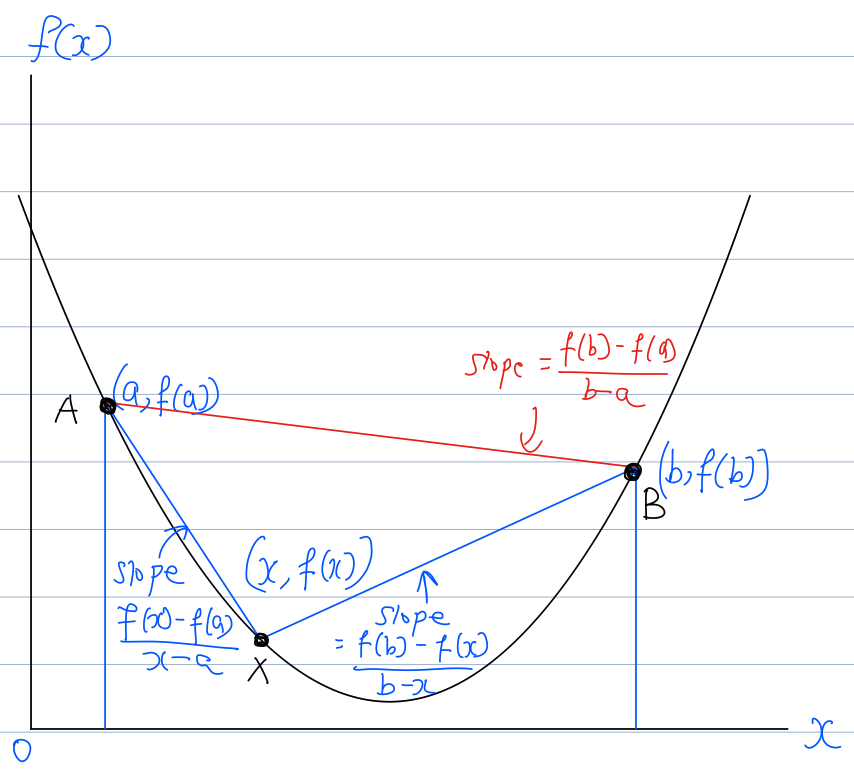
\includegraphics[width=0.5\textwidth]{images/graph.png}
    \caption{\label{fig:graph} The point X exists in the bound of $x \in (a,b)$ which can move freely from point A to B as shown in the figure. Each term in three inequalities determines the slope of a line. It is clear from the figure that the slope of line AX is always less than AB which is the actually the meaning of first two inequalities given in the problem. Similarly, the slope of line BX is always greater than line AB which is the meaning of last two inequalities. This is visual representation of how inequalities hold true.}
    \end{figure}
    \newpage
   \textbf{Proof:}
   \\
 
   First we will prove inequalities on left-side. Let $t = \frac{x-a}{b-a}$. Given that $x \in (a,b)$ and $a < b$, we can say $0 < t < 1$. Let's rewrite $f(x)$ as following:-
    \begin{equation}
       \begin{split}
       f(x) & = f(a + x - a) \\
       & = f(a + \frac{x-a}{b-a}(b-a)) \\
       & = f(a + t(b-a)) \\
       & = f(tb + a - ta) \\
       & = f(tb + (1-t)a) \\ 
       & \leq tf(b) + (1-t)f(a) \hspace{2em} \text{[According to the convexity property]} \\
       & \leq tf(b) + f(a) - tf(a) \\
       \Rightarrow f(x) - f(a) & \leq tf(b) - tf(a) \hspace{2em} \text{[Subtracting f(a) from both sides]} \\
       \Rightarrow \frac{f(x) - f(a)}{x-a} & \leq \frac{tf(b) - tf(a)}{x-a} \hspace{2em} \text{[Diving both side by x - a]} \\
       & \leq \frac{t}{x-a}(f(b) - f(a)) \\
       & \leq \frac{f(b) - f(a)}{b-a} \hspace{2em} \text{[Because $t = \frac{x-a}{b-a}$]}
       \end{split} 
   \end{equation}
   Similarly, we will prove inequalities on right-side. Let $t = \frac{b-x}{b-a}$. Given that $x \in (a,b)$ and $a < b$, we can say $0 < t < 1$. Let's rewrite $f(x)$ as following:-
    \begin{equation}
       \begin{split}
       f(x) & = f(b + x - b) \\
       & = f(b + \frac{x-b}{b-a}(b-a)) \\
       & = f(b + \frac{b-x}{b-a}(a-b)) \\
       & = f(b + t(a-b)) \\
       & = f(ta + b - tb) \\
       & = f(ta + (1-t)b) \\ 
       & \leq tf(a) + (1-t)f(b) \hspace{2em} \text{[According to the convexity property]} \\
       & \leq tf(a) + f(b) - tf(b) \\
       \Rightarrow f(x) - f(b) & \leq tf(a) - tf(b) \hspace{2em} \text{[Subtracting f(b) from both sides]} \\
        \Rightarrow f(b) - f(x) & \geq tf(b) - tf(a) \hspace{2em} \text{[Multiplying -1 on both sides. This changes inequality.]} \\
       \Rightarrow \frac{f(b) - f(x)}{b-x} & \geq \frac{tf(b) - tf(a)}{b-x} \hspace{2em} \text{[Diving both side by b - x]} \\
       & \geq \frac{t}{b-x}(f(b) - f(a)) \\
       & \geq \frac{f(b) - f(a)}{b-a} \hspace{2em} \text{[Because $t = \frac{b-x}{b-a}$]} \\
       \Rightarrow \frac{f(b) - f(a)}{b-a} & \leq \frac{f(b) - f(x)}{b-x} 
       \end{split} 
   \end{equation}
   Putting eq(2) and (3) proof together, we get,
   \begin{equation}
       \frac{f(x) - f(a)}{x-a} \leq \frac{f(b) - f(a)}{b-a} \leq \frac{f(b) - f(x)}{b-x} 
   \end{equation}
   
    \newpage
    \begin{taskbox}
    \task{Q2 Linear Algebra [5 pts].}
    If $A$ and $B$ are positive definite matrices, prove that the matrix $\left[\begin{array}{c c} A  &0 \\ 0 &B \end{array} \right]$ is also positive definite. $0$'s here represent matrices of zeros of sufficient size to fill. 
    \end{taskbox}

    \\ \\ \textbf{Proof:}

    If A and B are positive definite then by definition we can say,
    \begin{equation}
    \begin{split}
        & x^{T}Ax > 0, \forall x \in \R^{n} \\
        & y^{T}Ay > 0, \forall y \in \R^{n} \\
    \end{split}
    \end{equation}
    If we add these equation, the inequalities still holds true, therefore we have,
    \begin{equation}
    \begin{split}
        & x^{T}Ax + y^{T}Ay > 0, \forall x \in \R^{n} \\
        & \left[\begin{array}{c c} x \\ y \end{array} \right]^T\left[\begin{array}{c c} A  &0 \\ 0 &B \end{array} \right]\left[\begin{array}{c c} x \\ y \end{array} \right] > 0 \\
        & z^T\left[\begin{array}{c c} A  &0 \\ 0 &B \end{array} \right]z > 0 \hspace{2em}  [z=\left[\begin{array}{c c} x \\ y \end{array} \right]].
    \end{split}
    \end{equation}
    It is clear that if $\forall x \in \R^{n}$ and  $\forall y \in \R^{n}$ then $\forall z \in \R^{2 \times n}$. Hence, given matrix is also a positive definite.
    \\
    \begin{taskbox}
    \task{Q3 Calculus I [10pts].}
    Compute the gradient $\nabla f(\mathbf{x})$ and Hessian $\nabla^2f(x)$ for the function 
    \begin{equation}
    f(\mathbf{x}) = (x_1 + x_2)(x_1x_2 + x_1 x_2^2)
    \label{eq:q3}
    \end{equation}
    Find at least three stationary points of this function  and compute the Hessian at each. Show that $\mathbf{x}=[3/8, -6/8]^T$ is a local maxima.
    \end{taskbox}
    \\ \\ \textbf{Proof:} \\
    Rewriting $f(x)$ and taking partial derivative with respect to $x_1$ and $x_2$ we get,
    \begin{equation}
        \begin{split}
            f(x) & = x_1^2x_2 + x_1^2x_2^2 + x_1x_2^2 + x_1x_2^3 \\
            \Rightarrow \frac{\delta f}{\delta x_1} & = 2x_1x_2 + 2x_1x_2^2 + x_2^2 + x_2^3 \\
            \Rightarrow \frac{\delta f}{\delta x_2} & = x_1^2 + 2x_1^2x_2 + 2x_1x_2 + 3x_1x_2^2
        \end{split}
    \end{equation}
    Recomputing partial derivative of $\frac{\delta f}{\delta x_1}$ and $\frac{\delta f}{\delta x_2}$ with respect to $x_1$ and $x_2$ we get,
    \begin{equation}
        \begin{split}
            \Rightarrow \frac{\delta^2f}{\delta x_1^2} & = 2x_2 + 2x_2^2 \\
            \Rightarrow \frac{\delta^2f}{\delta x_1x_2} & = 2x_1 + 4x_1x_2 + 2x_2 + 3x_2^2 \\
            \Rightarrow \frac{\delta^2f}{\delta x_2x_1} & = 2x_1 + 4x_1x_2 + 2x_2 + 3x_2^2 \\
            \Rightarrow \frac{\delta^2f}{\delta x_2^2} & = 2x_1 + 2x_1 + 6x_1x_2 \\
        \end{split}
    \end{equation}
    Therefore,
    \begin{equation}
        \begin{split}
            \nabla f(\mathbf{x}) & =\left[\begin{array}{c c} \frac{\delta f}{\delta x_1} \\ \frac{\delta f}{\delta x_2} \end{array} \right] \\
            & = \left[\begin{array}{c c} 2x_1x_2 + 2x_1x_2^2 + x_2^2 + x_2^3 \\ x_1^2 + 2x_1^2x_2 + 2x_1x_2 + 3x_1x_2^2 \end{array} \right] 
        \end{split}
    \end{equation}
    and Hessian is given by,
    \begin{equation}
        \begin{split}
          Hessian \nabla^2f(x) & = \left[\begin{array}{c c} \frac{\delta^2f}{\delta x_1^2} &\frac{\delta^2f}{\delta x_1x_2}  \\  \frac{\delta^2f}{\delta x_2x_1}  &\frac{\delta^2f}{\delta x_2^2} \end{array} \right] \\
          Hessian \nabla^2f(x) & = \left[\begin{array}{c c} 2x_2 + 2x_2^2  &2x_1 + 4x_1x_2 + 2x_2 + 3x_2^2  \\  2x_1 + 4x_1x_2 + 2x_2 + 3x_2^2  &2x_1 + 2x_2 + 6x_1x_2 \end{array} \right]
        \end{split}
    \end{equation}
    To compute the stationary points of this function, let's equate gradient to zero and find $x_1$, $x_2$, and f(x) for each.
    \begin{equation}
        \begin{split}
          & \nabla f(\mathbf{x}) = 0 \\
          & \Rightarrow \left[\begin{array}{c c} 2x_1x_2 + 2x_1x_2^2 + x_2^2 + x_2^3 \\ x_1^2 + 2x_1^2x_2 + 2x_1x_2 + 3x_1x_2^2 \end{array} \right] = 0 \\
        \end{split}
    \end{equation}
    To solve this non-linear equation, let's get rid of higher order variables 
    \begin{equation}
        \begin{split}
           & (2x_1x_2 + 2x_1x_2^2 + x_2^2 + x_2^3 = 0) \times 3x_1\\
          & (x_1^2 + 2x_1^2x_2 + 2x_1x_2 + 3x_1x_2^2 = 0) \times y \\
          & \Rightarrow \\
          & 6x_1^2x_2 + 6x_1^2x_2^2 + 3x_1x_2^2 + 3x_1x_2^3 = 0 \\
          & -x_1^2x_2 - 2x_1^2x_2^2 - 2x_1x_2^2 - 3x_1x_2^3 = 0 \\
          & \mathclap{\rule{6cm}{0.4pt}}\\
          & 5x_1^2x_2 + 4x_1^2x_2^2 + x_1^2 = 0 \\ 
          & \Rightarrow x_1x_2(5x_1 + 4x_1x_2 + x_2) = 0 
        \end{split}
    \end{equation}
    \begin{equation}
        \Rightarrow x_1x_2 = 0 
    \end{equation}
    or,
    \begin{equation}
        \Rightarrow 5x_1 + 4x_1x_2 + x_2 = 0 
    \end{equation}
    From equation 14, we can say $x_1 = 0$ and putting that in equation 15, we get $x_2 = 0$ which is our first solution. If we put $x_1 = 0$ in equation 12 (first equation), we get,
    \begin{equation}
        \begin{split}
            & \Rightarrow x_2^2 + x_2^3 = 0 \\ 
            & \Rightarrow x_2^2(1 + x_2) = 0 \\
            & \Rightarrow x_2 = -1 \\
        \end{split}
    \end{equation}
    which is our second solution. Again using equation 12, and getting rid of lower order variables, we get,
    \begin{equation}
        \begin{split}
           & (2x_1x_2 + 2x_1x_2^2 + x_2^2 + x_2^3 = 0) \times -1/x_2\\
          & (x_1^2 + 2x_1^2x_2 + 2x_1x_2 + 3x_1x_2^2 = 0) \times 2/x_1 \\
          & \Rightarrow \\
          & - 2x_1 - 2x_1x_2 - x_2 - x_2^2 = 0 \\
          & 2x_1 + 4x_1x_2 + 4x_2 + 6x_2^2 = 0 \\
          & \mathclap{\rule{6cm}{0.4pt}}\\
          & 2x_1x_2 + 3x_2 + 5x_2 = 0 \\ 
          & x_2 = \frac{-3-2x_1}{5}
        \end{split}
    \end{equation}
    Substituting $x_2$ in equation 15, we get,
    \begin{equation}
        \begin{split}
          & 5x_1 + 4x_1(\frac{-3-2x_1}{5}) + (-3-2x_1)  = 0 \\
          & 8x_1 - 11x_1 + 3 = 0  \\
          & (8x_1-3)(x_1-1)=0 \\
          & \Rightarrow x_1 = \frac{3}{8}  \\
          & \Rightarrow x_1 = 1
        \end{split}
    \end{equation}
    Putting $x_1=3/8$ and $x_1=1$ in equation 15, we get $x_2=-6/8$ and $x_2=-1$ respectively. Keeping all solution together, we have following,
    \begin{center}
    \begin{tabular}{ | m{1em} | m{1em} | m{1cm} |  m{10em} | m{10em} | } 
      \hline
      $x_1$ & $x_2$ & $f(x)$ & Hessian $\Delta^2f(x)$ & $Det(\text{Hessian} \Delta^2f(x))$ \\ 
      \hline
      0 & -1 & 0 & $\left[\begin{array}{c c} 0  &1 \\ 1 &-2 \end{array} \right]$ & -1 \\ 
      \hline
      0 & 0 & 0 & $\left[\begin{array}{c c} 0  &0 \\ 0 &0 \end{array} \right]$ & 0 \\ 
      \hline
      $\frac{3}{8}$ &  $-\frac{6}{8}$ & $\frac{27}{1024}$ & $\left[\begin{array}{c c} -3/8  &-3/16 \\ -3/16 &-39/16 \end{array} \right]$ & 225/256 \\ 
      \hline
      1 & -1 & 0 & $\left[\begin{array}{c c} 0  &-1 \\ -1 &-6 \end{array} \right]$ & -5\\ 
      \hline
    \end{tabular}
    \end{center}
    From all stationary points, when $x_1 = 3/8$ and $y= -6/8$, the determinant of Hessian matrix provides the positive value so it must be either a local minima or maxima. Since corresponding $f_{xx}(x)$ (first row, first column of Hessian matrix) is negative, it is a local maxima because of negative concavity.
    \\
    \begin{taskbox}
    \task{Q4 Calculus II [10pts].}
    Show that the function 
    \begin{equation}
        f(\mathbf{x}) = 8x_1 + 12x_2 + x_1^2 - 2x^2_2
    \end{equation}
    has only one stationary point, and that it is not a minimum nor a maximum, but a saddle point.
    \end{taskbox}
    \\ \\ \textbf{Proof:} \\
    To find a solution, we equate  of $\nabla f(\mathbf{x})$ to zero.  Therefore,
    \begin{equation}
        \begin{split}
                & \nabla f(\mathbf{x}) = 0 \\
               \Rightarrow & \left[\begin{array}{c c} 8 + 2x_1 \\ 12-4x_2 \end{array} \right] = 0 \\
               \Rightarrow & \\
               & x_1 = -4, x_2 = 3, f(x) = 2
        \end{split}
    \end{equation}
    Computing Hessian $\Delta^2 f(x)$,
    \begin{equation}
        \begin{split}
          Hessian \nabla^2f(x) & = \left[\begin{array}{c c} \frac{\delta^2f}{\delta x_1^2} &\frac{\delta^2f}{\delta x_1x_2}  \\  \frac{\delta^2f}{\delta x_2x_1}  &\frac{\delta^2f}{\delta x_2^2} \end{array} \right] \\
          Hessian \nabla^2f(x) & = \left[\begin{array}{c c} 2  &0  \\ 0  &-4 \end{array} \right]
        \end{split}
    \end{equation}
    We can see we have only one stationary point. If we compute determinant of Hessian $\Delta^2 f(x)$, we get -8, which is negative and it means it is a saddle point.
    \newpage
    \begin{taskbox}
    \task{Q5 Graphs [5pts].}
    A \emph{topological order of a directed graph} $G=(V, E)$ is an ordering of its nodes such that for every edge $(v_i, v_j) \in E$, node $i$ appears in the ordering before node $j$. Prove that every directed acyclic graph (DAG) has a topological order. \\[5pt]
    
    \emph{Hint: A DAG always has at least one node with no incoming edges.}
    \end{taskbox}
    \\ \\ \textbf{Proof:} \\
    We can prove this by induction. Let G be DAG and $'n'$ represent number of nodes in G\\
    \begin{itemize}
        \item \textbf{Base case}:
        \\ If n = 1, then G is topological ordering
        \item \textbf{Induction hypothesis}:
        \\ $G'$ has topological ordering for $n' \leq n$ where $n'$ is number of nodes in $G'$
        \item \textbf{Induction step}:
        \\ We shall prove why it holds true for G with n+1 nodes.
        \\ We know that there is at least one node with no incoming edges in DAG. Let that node be $v$.
        \\ $G - \{v\}$ is also a DAG because removing $v$ from G does not create any cycles.
        \\ Since, now the number of nodes in $G$ becomes $n$, we can say $G$ has topological ordering according to induction hypothesis.
    \end{itemize}
    This proves the hypothesis.
\end{enumerate}

\section{Automatic Differentiation with Dynamic Computation Graphs}
\begin{enumerate}
   # Please refer to a code submission.
\end{enumerate}

\section{Debriefing}
\begin{enumerate}
    \item Approximately how many hours did you spend on this assignment?
    \\ - I spent around 20 hours.
    \item Would you rate it as easy, moderate, or difficult?
    \\ - It was moderate.
    \item Did you work on it mostly alone or did you discuss the problems with others?
    \\ - I did it all alone.
    \item How deeply do you feel you understand the material it covers (0\%–100\%)?
    \\ - I would say 95\%
    \item Any other comments?
    \\ - It was a good exercise in this assignment especially the math part. It's been a long time I looked back into what I studied in my undergrads. It never made sense 'where I would use this in my life' so it was easy to forgot. Realizing how important and empirical this is in deep learning and other engineering and science courses makes it interesting to learn.
\end{enumerate}

\end{document}
